Najniższy stopień automorfizmu przyjętego przez niezależny weryfikator: \textbf{6} (znane ograniczenie górne: $16$). Weryfikator sprawdza dokładnie, w arytmetyce liczb wymiernych, warunki $F(p_i)=q_i$, odwracalność (odwrotność wielomianowa o współczynnikach wymiernych) oraz stopień. Stopień ten jest ograniczeniem \emph{górnym}; o ograniczeniach dolnych mówią wyłącznie twierdzenia opisane w dalszych częściach raportu.

Przyjęte rozwiązania: 2; odrzucone: 0.
\begin{center}\small\begin{tabular}{rlp{5.2cm}p{5.6cm}}\toprule Stopień & Czynniki & Autor & Plik\\\midrule
6 & 2$\cdot$3 & iter01/zad3 & \texttt{praca/\allowbreak{}iter01/\allowbreak{}zad3/\allowbreak{}rozwiazanie\_6.json}\\
16 & 4$\cdot$4 & konstrukcja bazowa (skrypt przygotowany przed eksperymentem) & \texttt{praca/\allowbreak{}iter00/\allowbreak{}baza/\allowbreak{}rozwiazanie\_bazowe.json}\\
\bottomrule\end{tabular}\end{center}
\subsection*{Najlepsze znalezione odwzorowanie}
T1=(x,y+f(x)) z f st. 2 (punkty kwadratu parami o wspólnym x), T2=(x+g(y),y) z g st. 3 (D,E mają wspólne y po zmianie afinicznej), następnie afiniczne; stopień 2*3=6
\noindent $F = \varphi_n\circ\dots\circ\varphi_1$, gdzie (w kolejności działania):
\begin{align*}
\varphi_{1}&\colon (x,y)\mapsto\left(x,\ y + \left(\frac{8 x^{2}}{3} - 3 x - \frac{8}{3}\right)\right)\\\varphi_{2}&\colon (x,y)\mapsto\left(x + \left(\frac{y^{3}}{96} - \frac{y^{2}}{8} - \frac{25 y}{24} + \frac{1}{2}\right),\ y\right)\\\varphi_{3}&\colon (x,y)\mapsto\left(- \frac{x}{3},\ - x - y\right)
\end{align*}
Postać rozwinięta:
\begin{flushleft}\small
$F_1(x,y) = - \frac{16 x^{6}}{243} + \frac{2 x^{5}}{9} - \frac{2 x^{4} y}{27} + \frac{79 x^{4}}{324} + \frac{x^{3} y}{6} - \frac{293 x^{3}}{288} - \frac{x^{2} y^{2}}{36} + \frac{239 x^{2} y}{864} + \frac{493 x^{2}}{648} + \frac{x y^{2}}{32} - \frac{5 x y}{12} - \frac{35 x}{72} - \frac{y^{3}}{288} + \frac{5 y^{2}}{72} + \frac{11 y}{216} - \frac{355}{486}$\par\medskip
$F_2(x,y) = - \frac{16 x^{6}}{81} + \frac{2 x^{5}}{3} - \frac{2 x^{4} y}{9} + \frac{79 x^{4}}{108} + \frac{x^{3} y}{2} - \frac{293 x^{3}}{96} - \frac{x^{2} y^{2}}{12} + \frac{239 x^{2} y}{288} - \frac{83 x^{2}}{216} + \frac{3 x y^{2}}{32} - \frac{5 x y}{4} + \frac{37 x}{24} - \frac{y^{3}}{96} + \frac{5 y^{2}}{24} - \frac{61 y}{72} + \frac{77}{162}$
\end{flushleft}
\IfFileExists{gen/najlepsze.pdf}{\begin{figure}[h!]\centering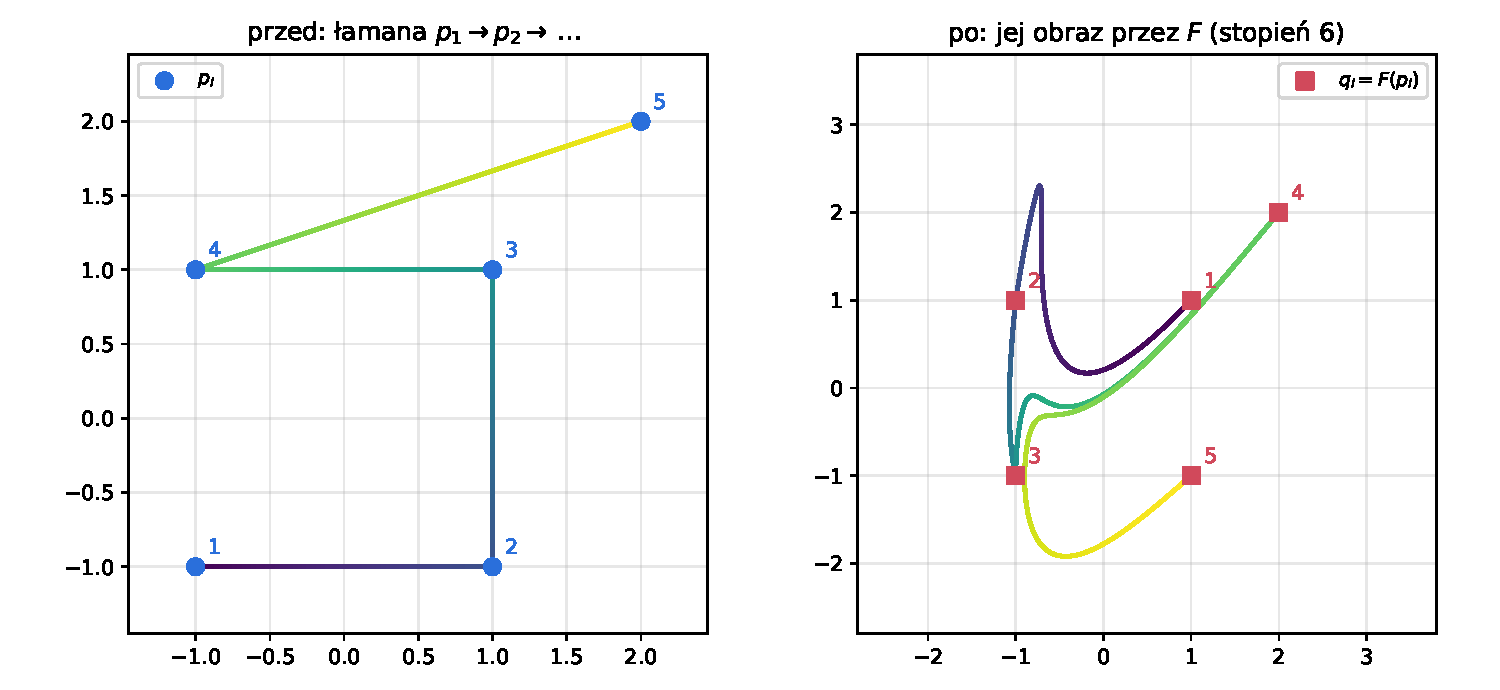
\includegraphics[width=\textwidth]{gen/najlepsze.pdf}\caption{Łamana $p_1\to\dots\to p_m$ (lewa) i jej obraz przez najlepsze znalezione $F$ (prawa); barwa wskazuje położenie wzdłuż łamanej.}\end{figure}}{}
\IfFileExists{gen/czynniki.pdf}{\begin{figure}[h!]\centering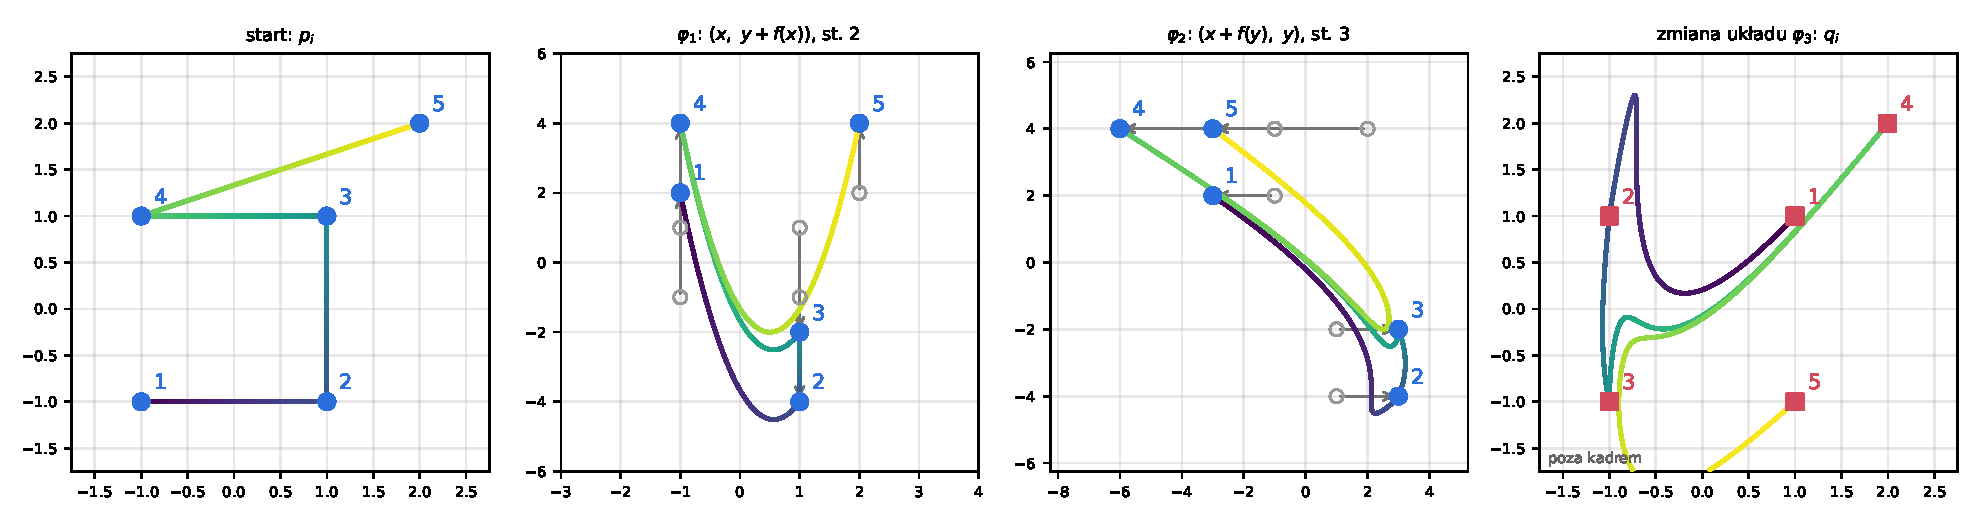
\includegraphics[width=\textwidth]{gen/czynniki.pdf}\caption{Działanie kolejnych czynników $\varphi_k$ najlepszego $F$ na punkty i łamaną. Czynnik trójkątny przesuwa punkty tylko pionowo albo tylko poziomo; każdy panel ma własny kadr.}\end{figure}}{}
\IfFileExists{gen/postep.pdf}{\begin{figure}[h!]\centering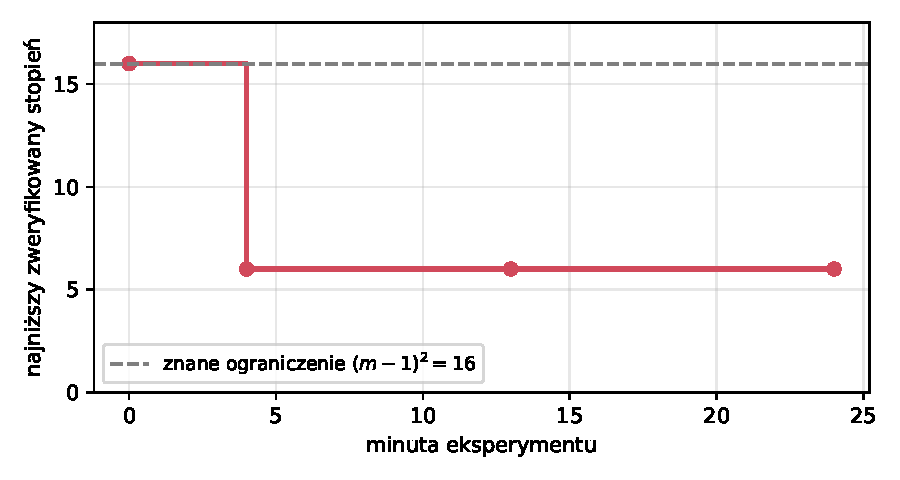
\includegraphics[width=0.7\textwidth]{gen/postep.pdf}\caption{Najniższy zweryfikowany stopień w kolejnych minutach eksperymentu.}\end{figure}}{}
